\documentclass[10pt]{book}
\usepackage[sectionbib]{natbib}
\usepackage{array,epsfig,fancyhdr,rotating}
\usepackage[driverfallback=dvipdfm]{hyperref}
\usepackage{epstopdf}
%%%%%%%%%%%%%%%%%%%%%%%%%%%%%%%%%%%%%%%%%%%%%%%%%%%%%%%%%%%%%%%%%%%%%%%%%%%%%%%%%%%%%%%%%%%%%%%%%%%%%%%%%%%%%%%%%%%%%%%%%%%%

\textwidth=31.9pc
\textheight=46.5pc
\oddsidemargin=1pc
\evensidemargin=1pc
\headsep=15pt
%\headheight=.2cm
\topmargin=.6cm
\parindent=1.7pc
\parskip=0pt


\usepackage{amsmath}
\usepackage{amssymb}
\usepackage{amsfonts}
\usepackage{amsthm}
\usepackage[export]{adjustbox}

\setcounter{page}{1}
\newtheorem{theorem}{Theorem}
\newtheorem{lemma}{Lemma}
\newtheorem{corollary}{Corollary}
\newtheorem{proposition}{Proposition}
\theoremstyle{definition}
\newtheorem{definition}{Definition}
%\newtheorem{proof}{Proof}
\newtheorem{example}{Example}
\newtheorem{remark}{Remark}
\pagestyle{fancy}

% Reference labels in the online appendix
\usepackage{xr}
\externaldocument{mdi}

%%%%%%%%%%%%%%%%%%%%%%%%%%%%%%%%%%%%%%%%%%%%%%%%%%%%%%%%%%%%%%%%%%%%%%%%%%%%%%%%%%%%%%%%%%%%%%%%%%%%%%%%%%%%%%%%%%%%%%%%%%%%
\pagestyle{fancy}
\def\n{\noindent}
\lhead[\fancyplain{} \leftmark]{}
\chead[]{}
\rhead[]{\fancyplain{}\rightmark}
\cfoot{}
\renewcommand{\headrulewidth}{0pt}

%%%%%%%%%%%%%%%%%%%%%%%%%%%%%%%%%%%%%%%%%%%%%%%%%%%%%%%%%%%%%%%%%%%%%%%%%%%%%%%%%%%%%%%%%%%%%%%%%%%%%%%%%%%%%%%%%%%%%%%%%%%%
%%%%%%%%%%%%%%%%%%%%%%%%%%%%%%%%%%%%%%%%%%%%%%%%%%%%%%%%%%%%%%%%%%%%%%%%%%%%%%%%%%%%%%%%%%%%%%%%%%%%%%%%%%%%%%%%%%%%%%%%%%%%

\begin{document}
\pagestyle{empty} % get rid of headers
%%%%%%%%%%%%%%%%%%%%%%%%%%%%%%%%%%%%%%%%%%%%%%%%%%%%%%%%%%%%%%%%%%%%%%%%%%%%%%%%%%%%%%%%%%%%%%%%%%%%%%%%%%%%%%%%%%%%%%%%%%%%
%%%%%%%%%%%%%%%%%%%%%%%%%%%%%%%%%%%%%%%%%%%%%%%%%%%%%%%%%%%%%%%%%%%%%%%%%%%%%%%%%%%%%%%%%%%%%%%%%%%%%%%%%%%%%%%%%%%%%%%%%%%%

\renewcommand{\baselinestretch}{2}

%\markright{ \hbox{\footnotesize\rm Statistica Sinica: Supplement
%%{\footnotesize\bf 24} (201?), 000-000
%}\hfill\\[-13pt]
%\hbox{\footnotesize\rm
%%\href{http://dx.doi.org/10.5705/ss.20??.???}{doi:http://dx.doi.org/10.5705/ss.20??.???}
%}\hfill }

\markboth{\hfill{\footnotesize\rm JASON POULOS AND RAFAEL VALLE} \hfill}
{\hfill {\footnotesize\rm MISSING DATA IMPUTATION} \hfill}

\renewcommand{\thefootnote}{}
$\ $\par \fontsize{12}{14pt plus.8pt minus .6pt}\selectfont

%%%%%%%%%%%%%%%%%%%%%%%%%%%%%%%%%%%%%%%%%%%%%%%%%%%%%%%%%%%%%%%%%%%%%%%%%%%%%%%%%%%%%%%%%%%%%%%%%%%%%%%%%%%%%%%%%%%%%%%%%%%%

 \centerline{\large\bf MISSING DATA IMPUTATION FOR SUPERVISED LEARNING}
%\vspace{2pt}
% \centerline{\large\bf FOR SUPERVISED CLASSIFICATION}
%\vspace{2pt}
% \centerline{\large\bf IF THIRD LINE IS NEEDED}
\vspace{.25cm}
% \author{Author(s)}
% \centerline{Jason Poulos and Rafael Valle} \vspace{.4cm} 
%\vspace{.4cm}
% \centerline{\it University of California, Berkeley}
\vspace{.55cm}
 \centerline{\bf Supplementary Material}
\vspace{.55cm}
\fontsize{9}{11.5pt plus.8pt minus .6pt}\selectfont
\noindent
This file contains descriptive plots of feature correlation and missing data patterns in the benchmark datasets; plots of Bayesian hyperparameter optimization for training ANNs; and test set error plots for classifiers trained on MNAR-perturbed data. 
\par

\setcounter{section}{0}
\setcounter{equation}{0}
\def\theequation{S\arabic{section}.\arabic{equation}}
\def\thesection{S\arabic{section}}

\fontsize{12}{14pt plus.8pt minus .6pt}\selectfont



\newpage
\lhead[\footnotesize\thepage\fancyplain{}\leftmark]{}\rhead[]{\fancyplain{}\rightmark\footnotesize\thepage}%Put this line in Page 2
\section{Descriptive plots}

\begin{figure}[h!]
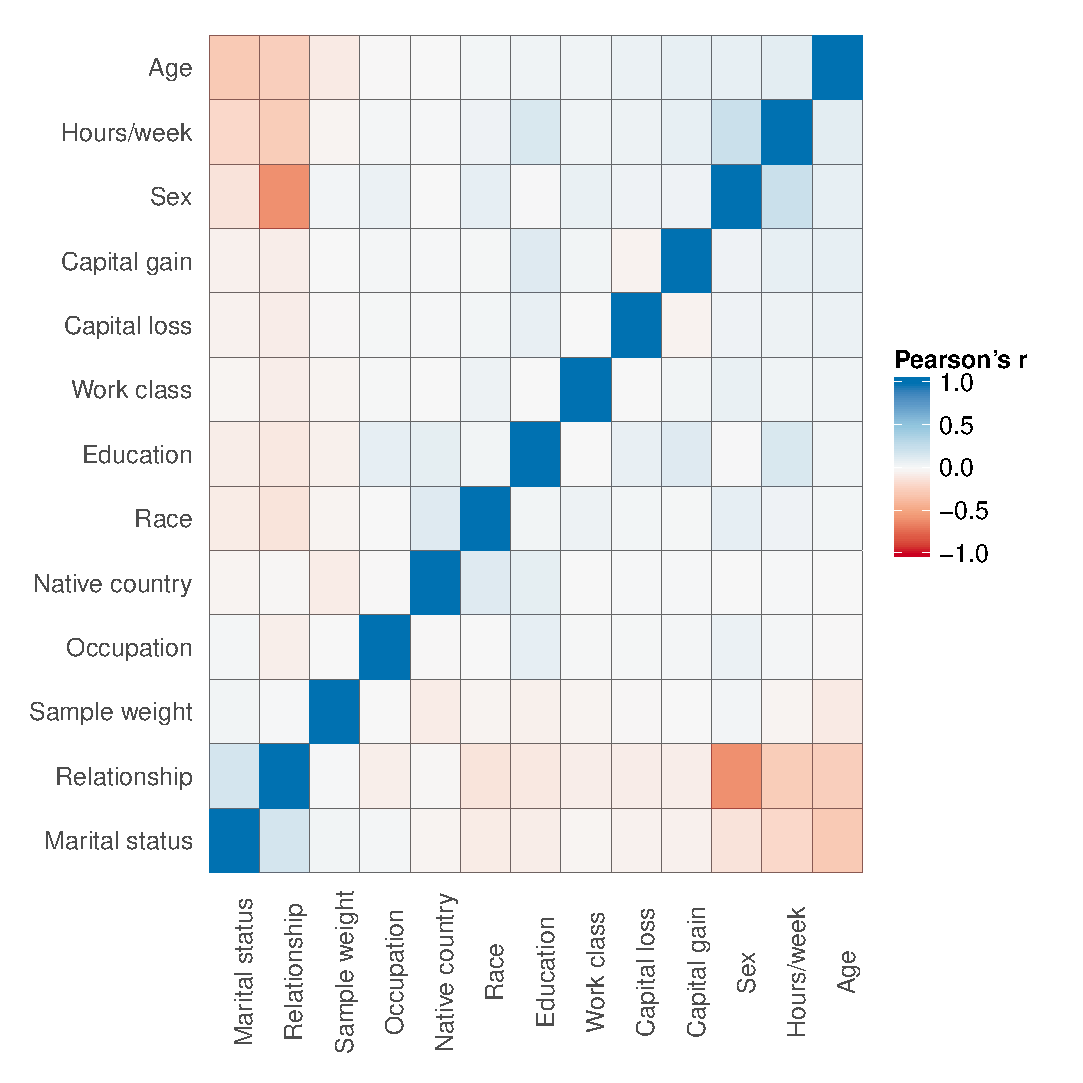
\includegraphics [scale=0.75, center]{figure/correlation-adult}\par
\caption{\footnotesize Correlation matrix for Adult training set. Pearsoepsn product-moment correlation coefficients (Pearson's r) are computed with listwise-deletion of missing values.}
 \label{fig:correlation-adult}
\end{figure}

\begin{figure}[h!]
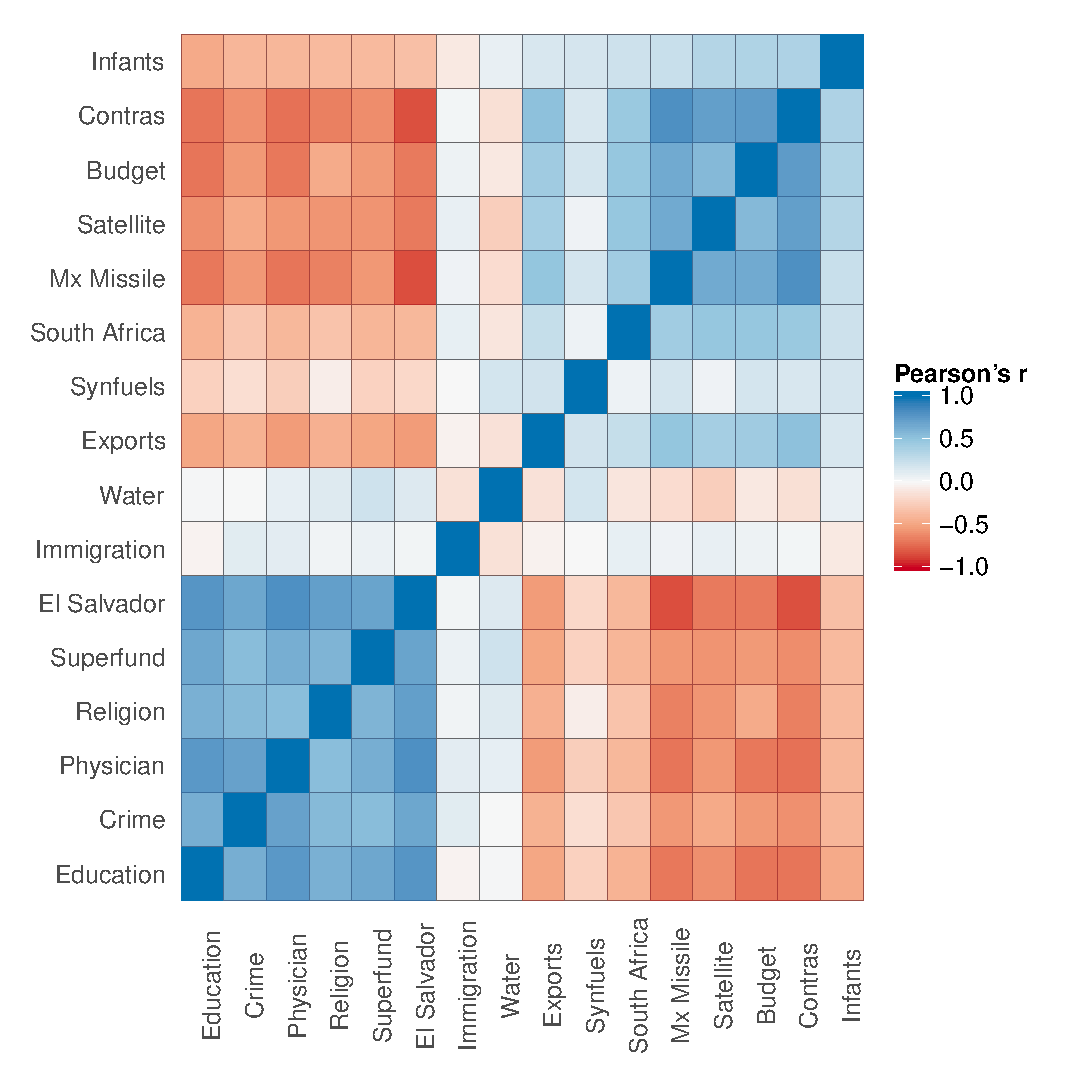
\includegraphics [scale=0.75, center]{figure/correlation-votes}\par
\caption{\footnotesize Correlation matrix for CVRs training set. See footnotes for Figure \ref{fig:correlation-adult}.}
 \label{fig:correlation-votes}
\end{figure}

\begin{figure}[h!]
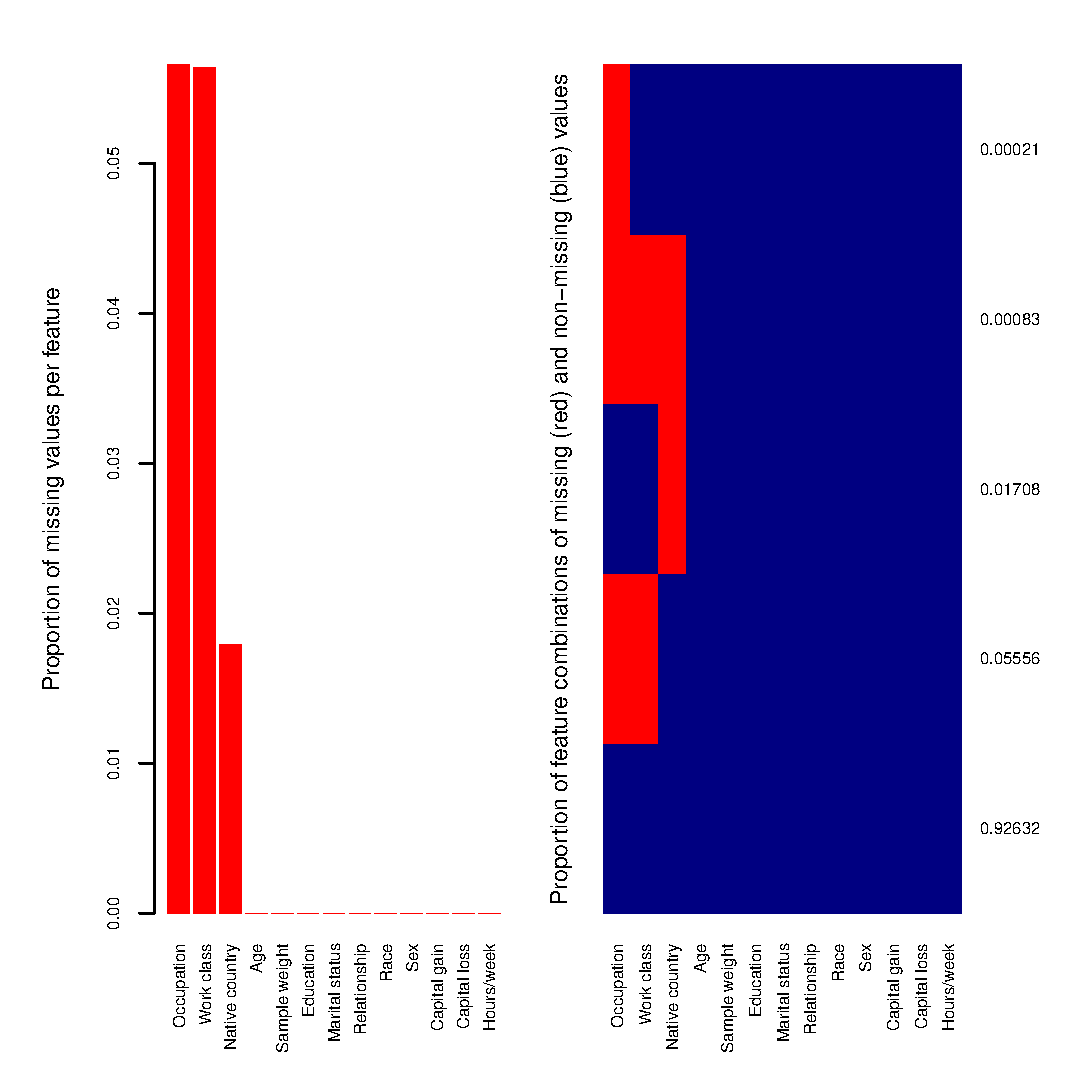
\includegraphics [scale=0.75, center]{figure/proportion-missing-adult}\par
\caption{\footnotesize Histogram of proportion of missing values in each feature (Left) of Adult training set and aggregation plot of all existing combinations of missing and non-missing values in the samples (Right).}
 \label{fig:proportion-missing-adult}
\end{figure}

\begin{figure}[h!]
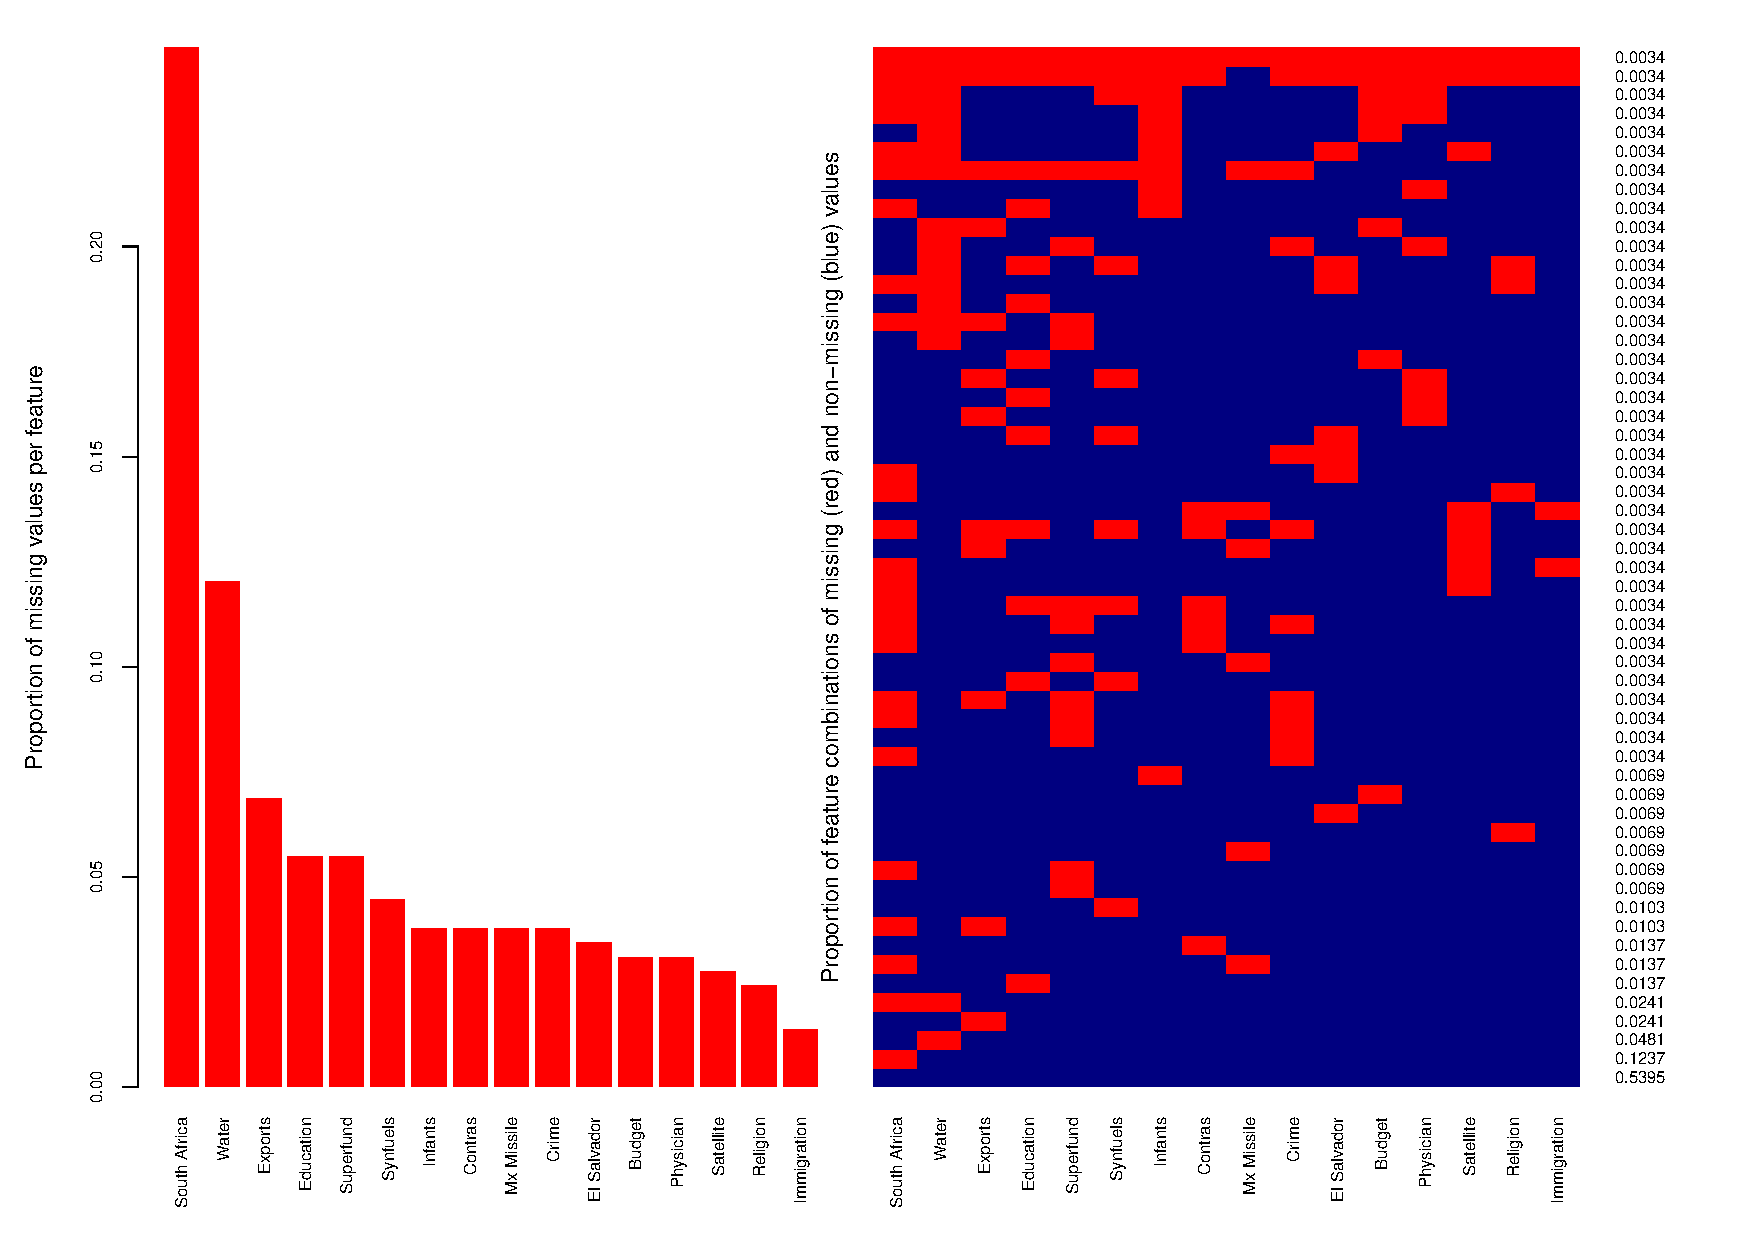
\includegraphics [scale=0.75, center]{figure/proportion-missing-votes}\par
\caption{\footnotesize Histogram of proportion of missing values in each feature (Left) of CVRs training set and aggregation plot of all existing combinations of missing and non-missing values in the samples (Right).}
 \label{fig:proportion-missing-votes}
\end{figure}

\clearpage
\section{Bayesian hyperparameter optimization}
\setcounter{equation}{0}

The goal of Bayesian optimization is to choose a point in the hyperparameter space that appropriately balances information gain and exploitation. Figure \ref{fig:params} shows the exploration of hyperparameter space during Bayesian optimization for both Adult and CVRs datasets. Each circle represents a candidate ANNs classifier trained on a differently imputed and perturbed dataset. More circles appear in the plot for CVRs simply due to the fact that the training set is smaller. We see that most of the candidate models use dropout and have an initial learning rate close to the maximum of 0.01. The plurality of candidate models appear to either have momentum (1) or not (0).

\begin{figure}[h!]
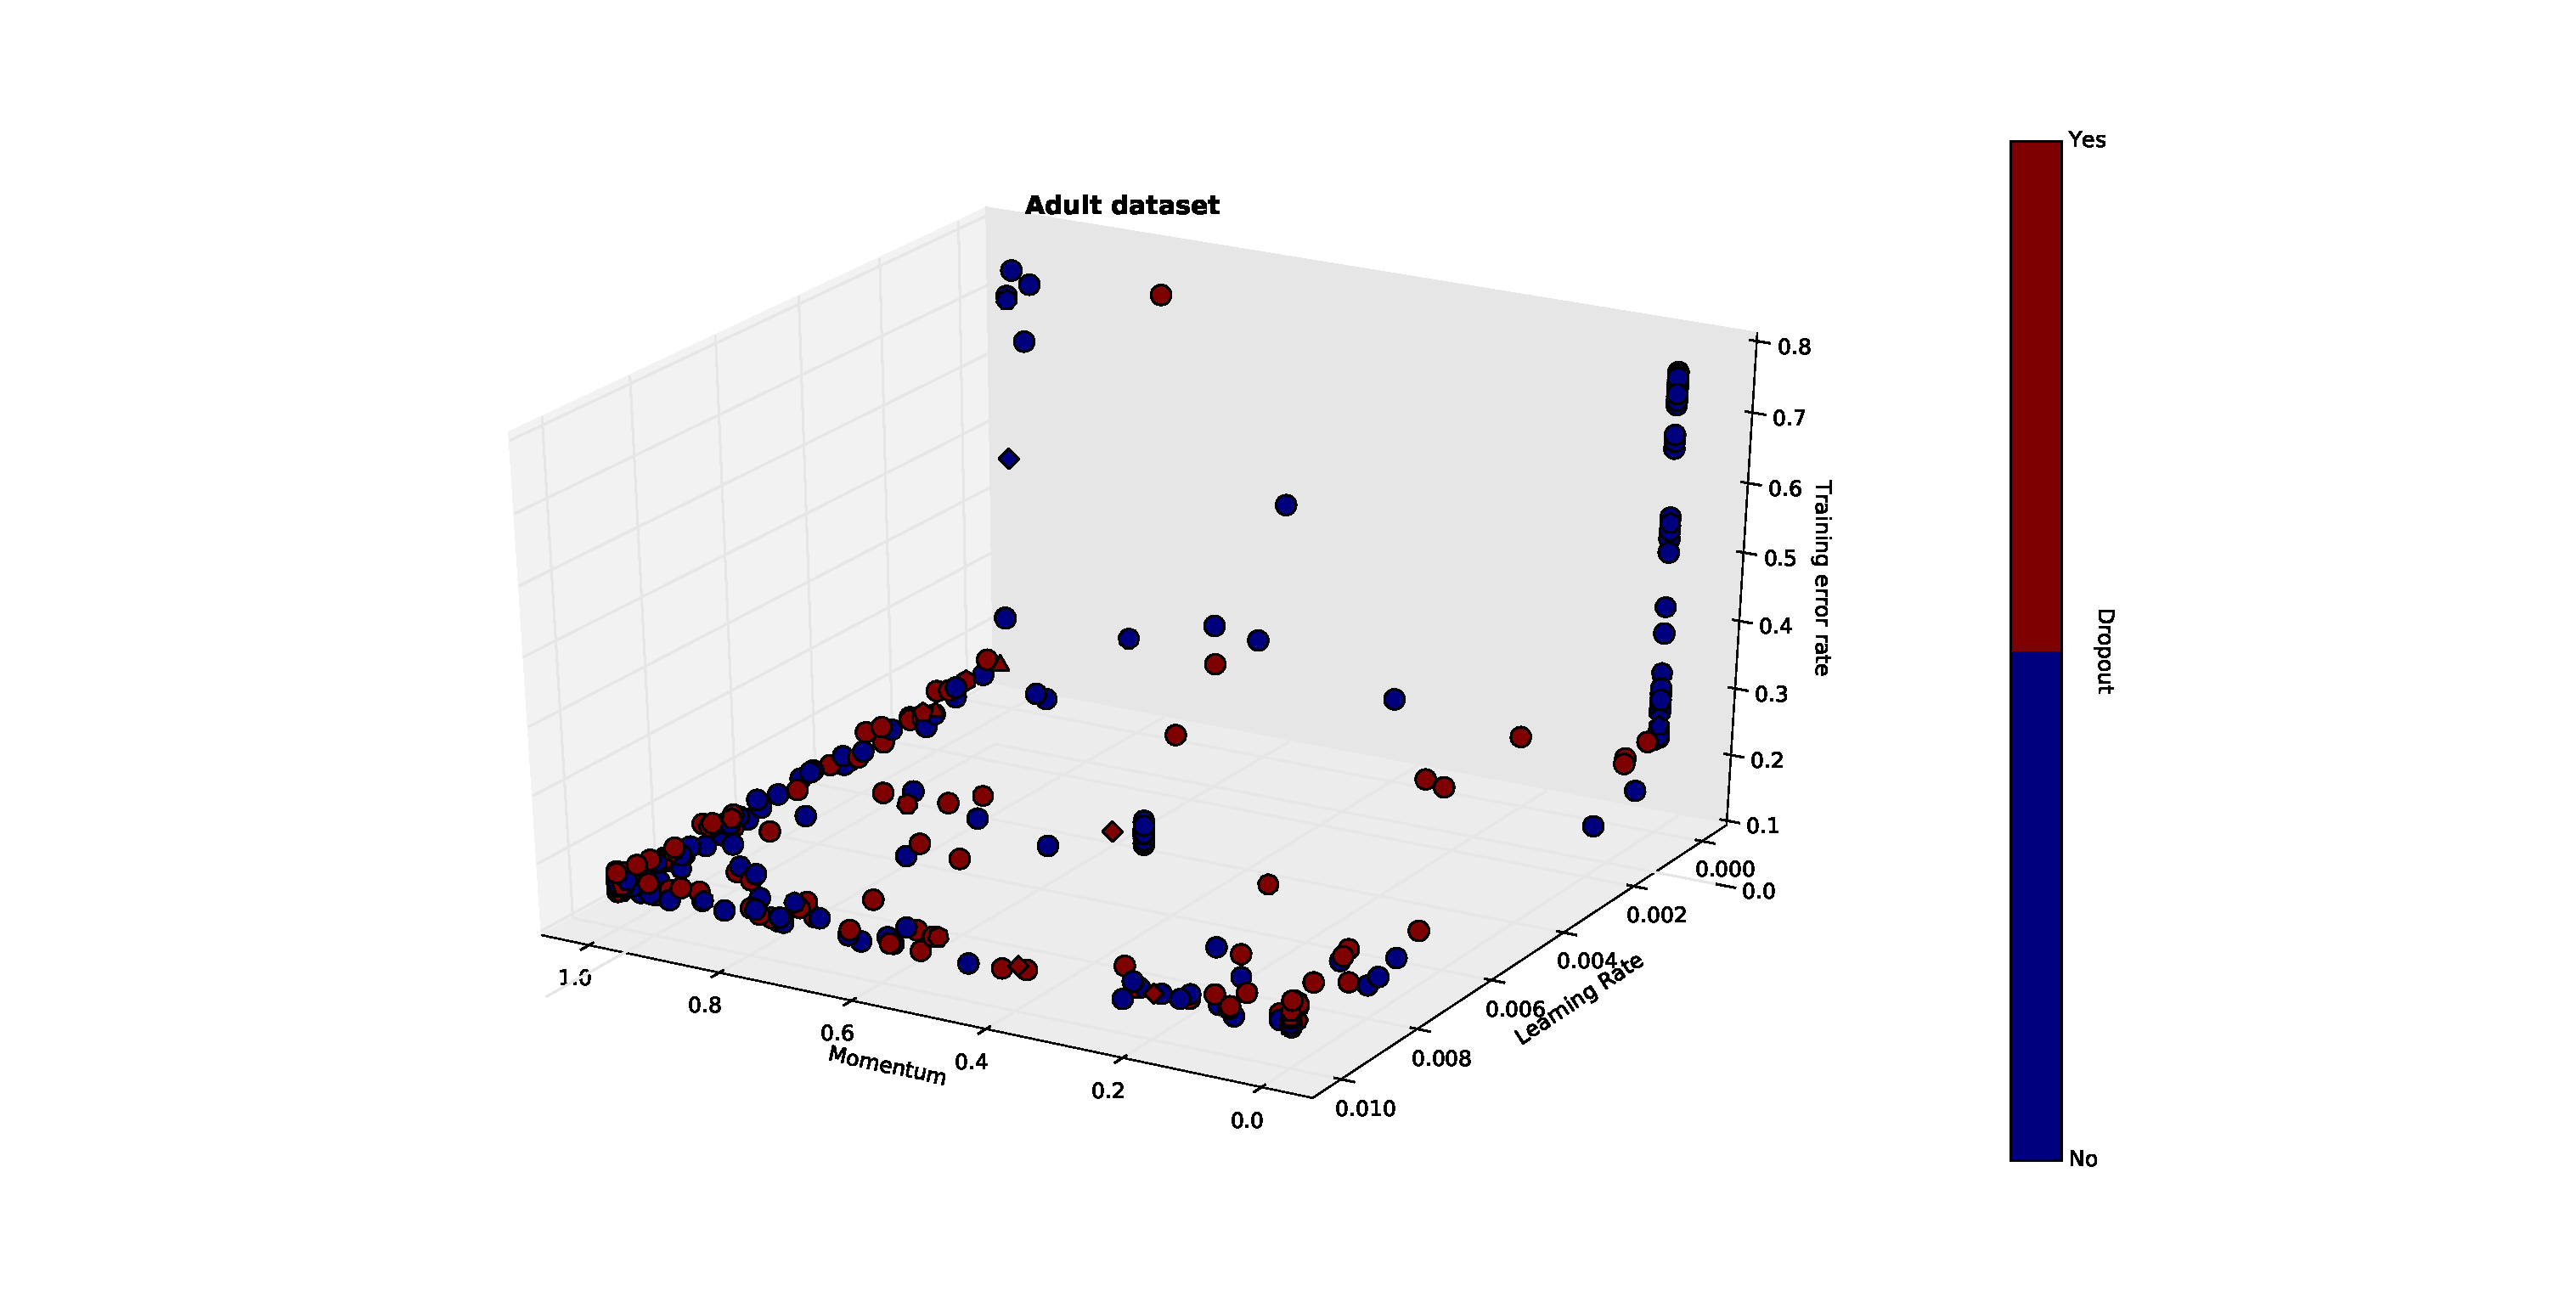
\includegraphics [scale=0.4, center, center]{figure/params3d_adult.eps}\par
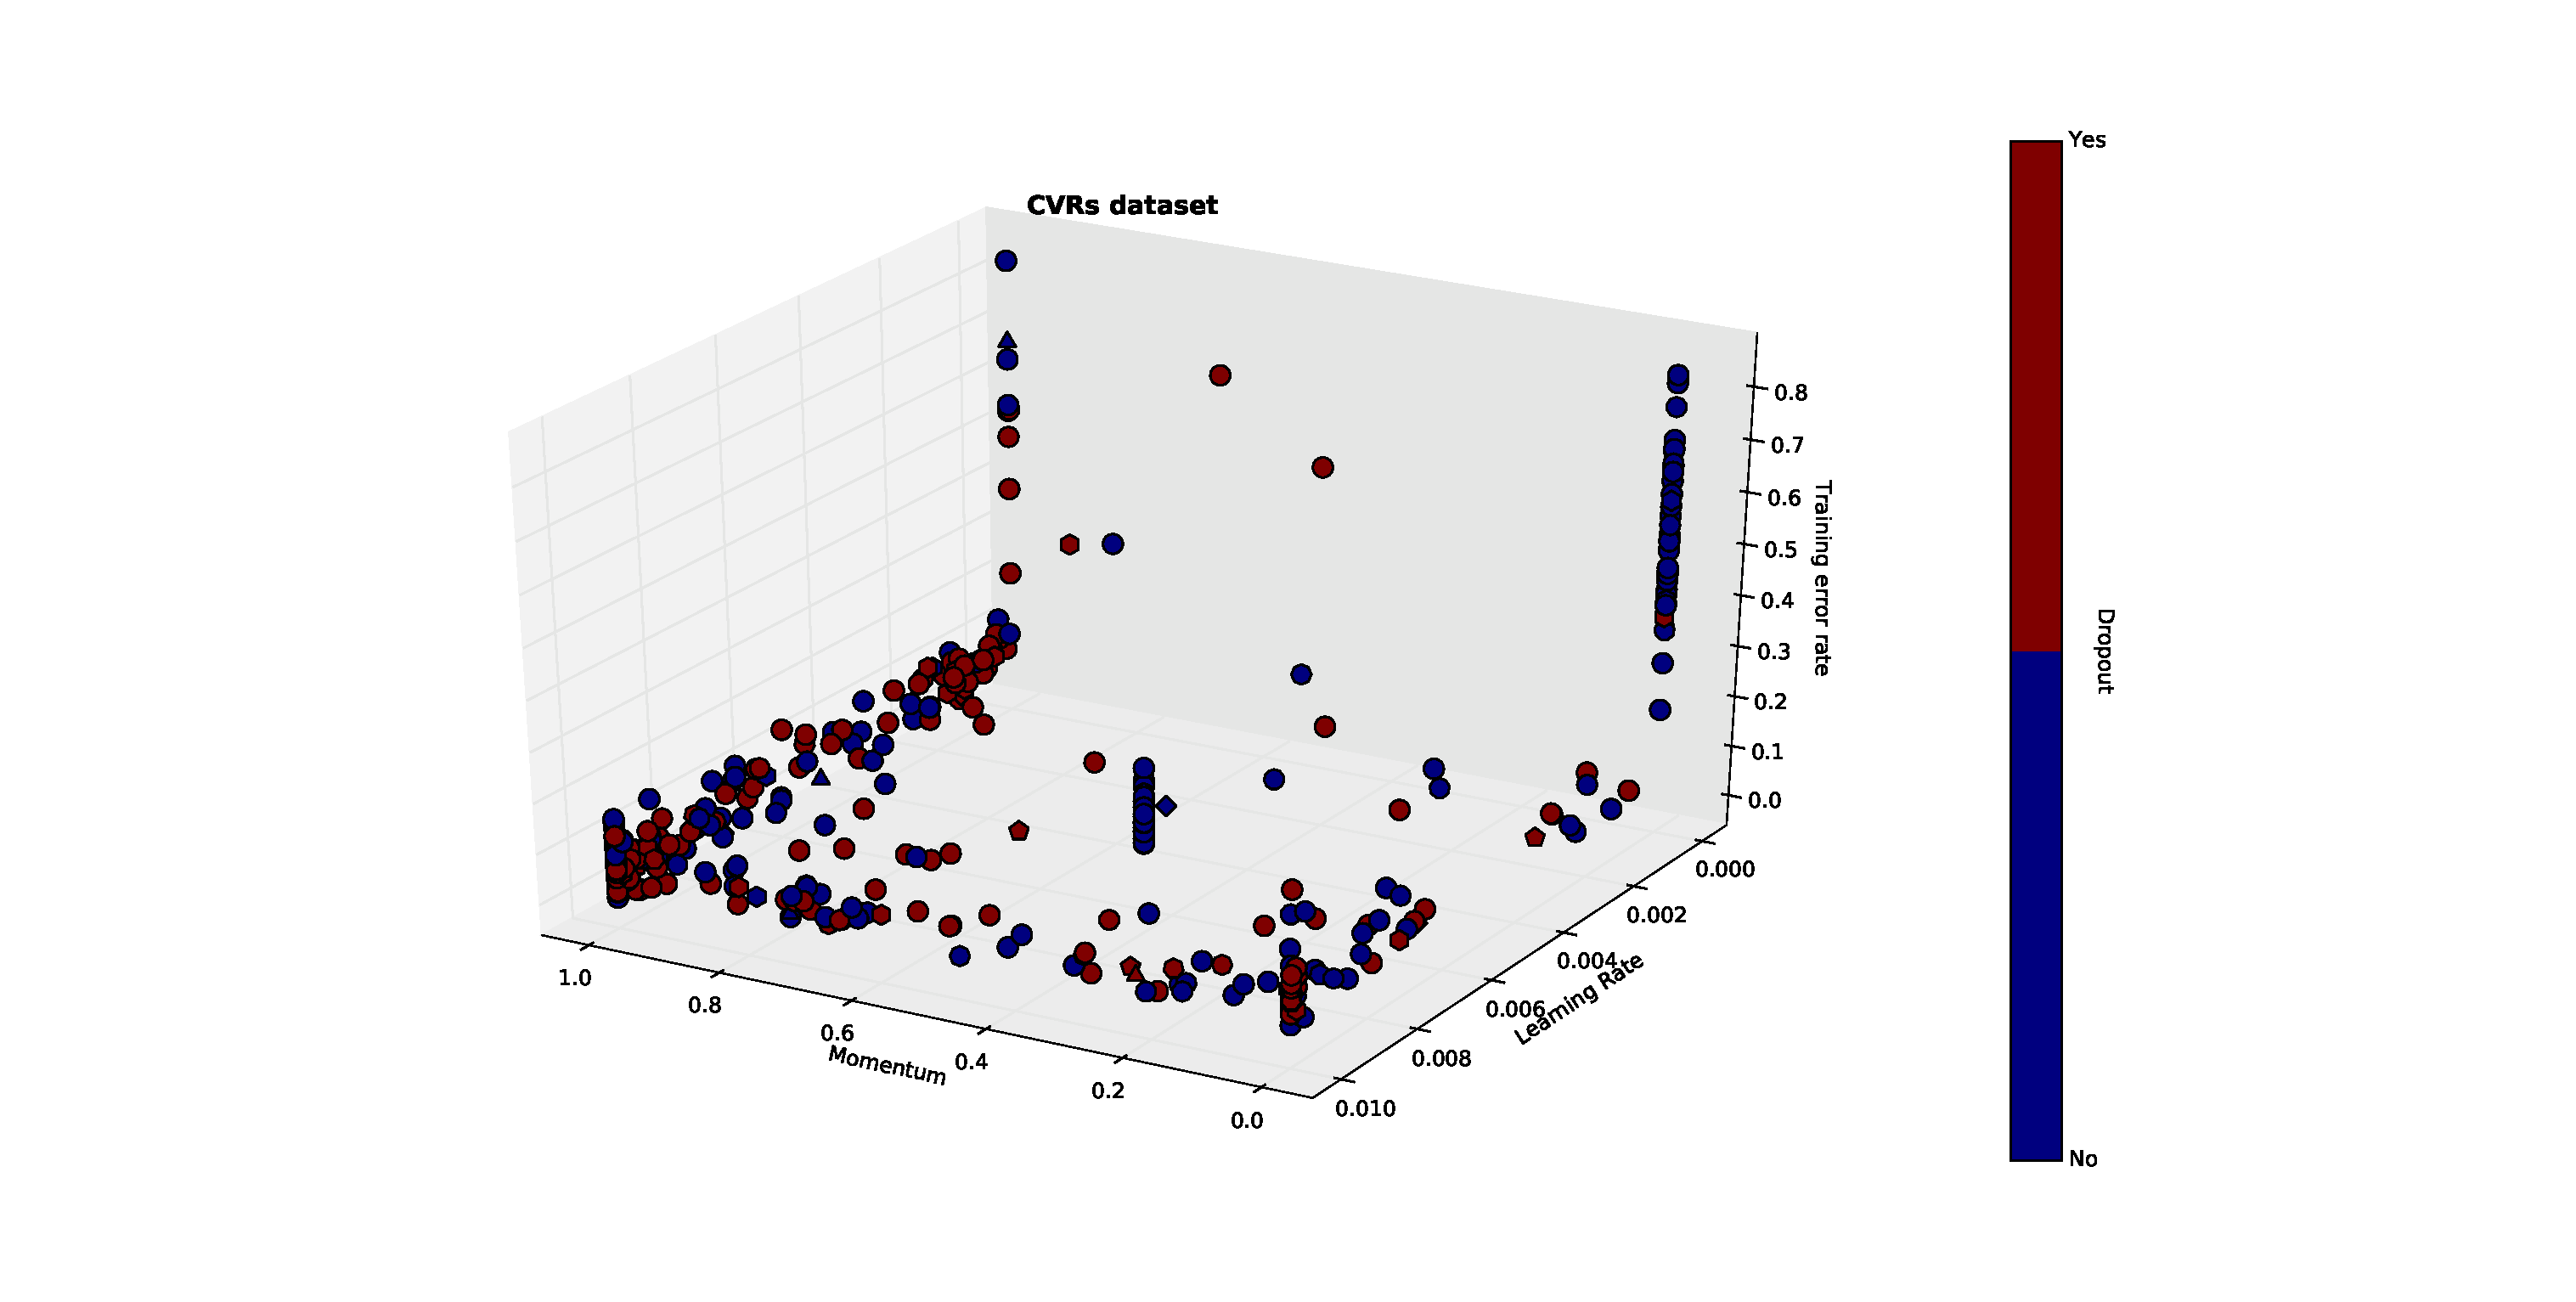
\includegraphics [scale=0.4, center, center]{figure/params3d_votes.eps}\par
\caption{\footnotesize Exploration of hyperparameter space during Bayesian optimization. Each circle represents a candidate ANNs classifier trained on a differently imputed and perturbed dataset.}
   \label{fig:params}
\end{figure}

\clearpage
\section{Results with MNAR perturbation}
\setcounter{equation}{0}

We perturb the training data according to the MNAR mechanism
 
 \begin{equation}\label{3.1}
\Pr (M_{ij} = 1 | y_{ij}, \phi) = \begin{cases}
\delta, &\text{if $y_{ij} \in A$}  \\
0, &\text{otherwise},
\end{cases}
\end{equation} where $A$ is a vector containing at least one value from each categorical feature that we determine likely to be missing. We select categorical values in the Adult dataset that are theoretically correlated with low socioeconomic status, such as the values ``Without pay'' and ``Never worked" for the feature \emph{Work class}. The existing literature suggests item nonresponse in surveys is correlated with low income and low education (Rubin et al., 1995). We include in $A$ only ``nay'' votes, under the assumption that refusing to take position on an issue or missing a vote is akin to voting against the issue. 

\begin{figure}[h!]
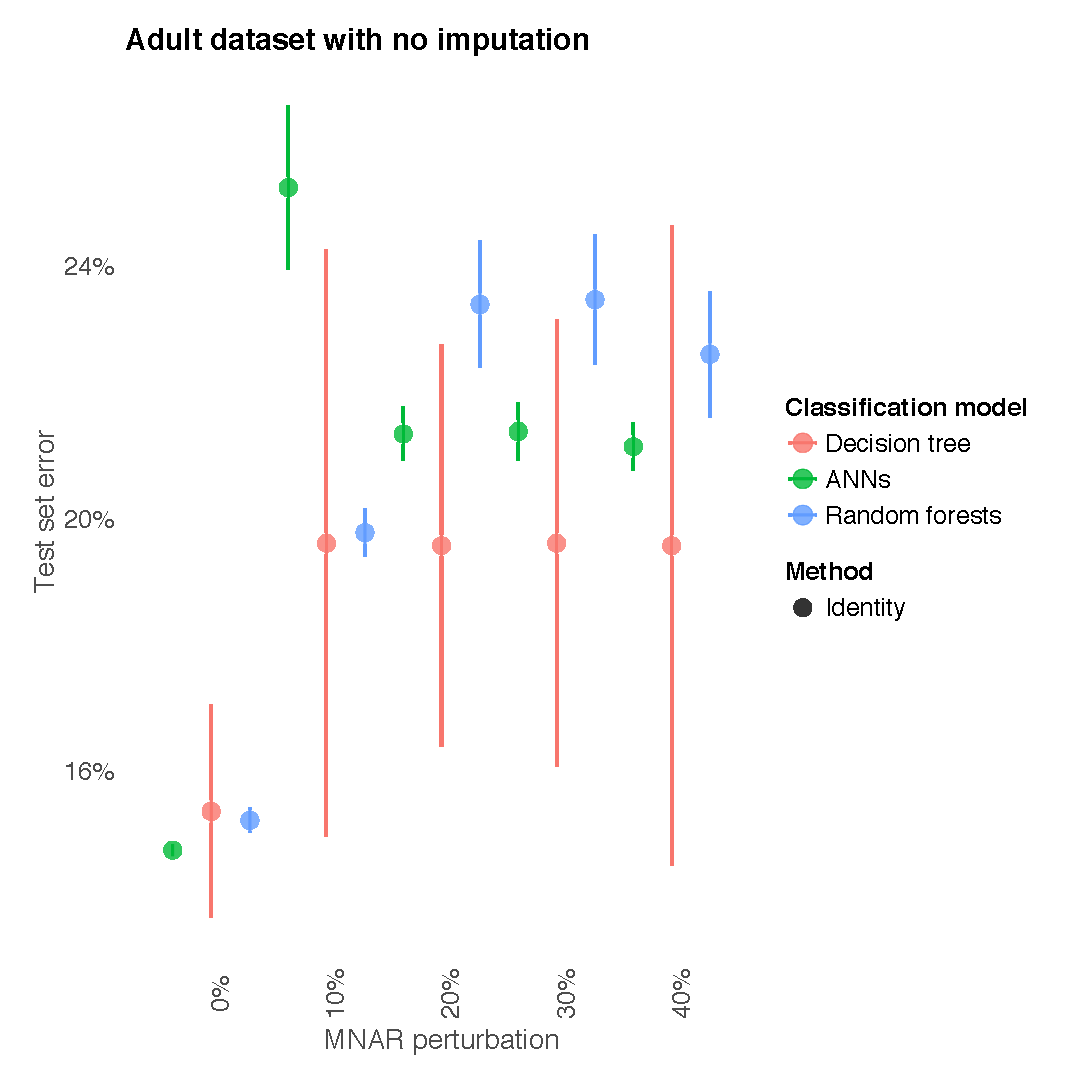
\includegraphics[scale=0.55, center]{figure/test-errors-adult-no-imp-mnar}\par
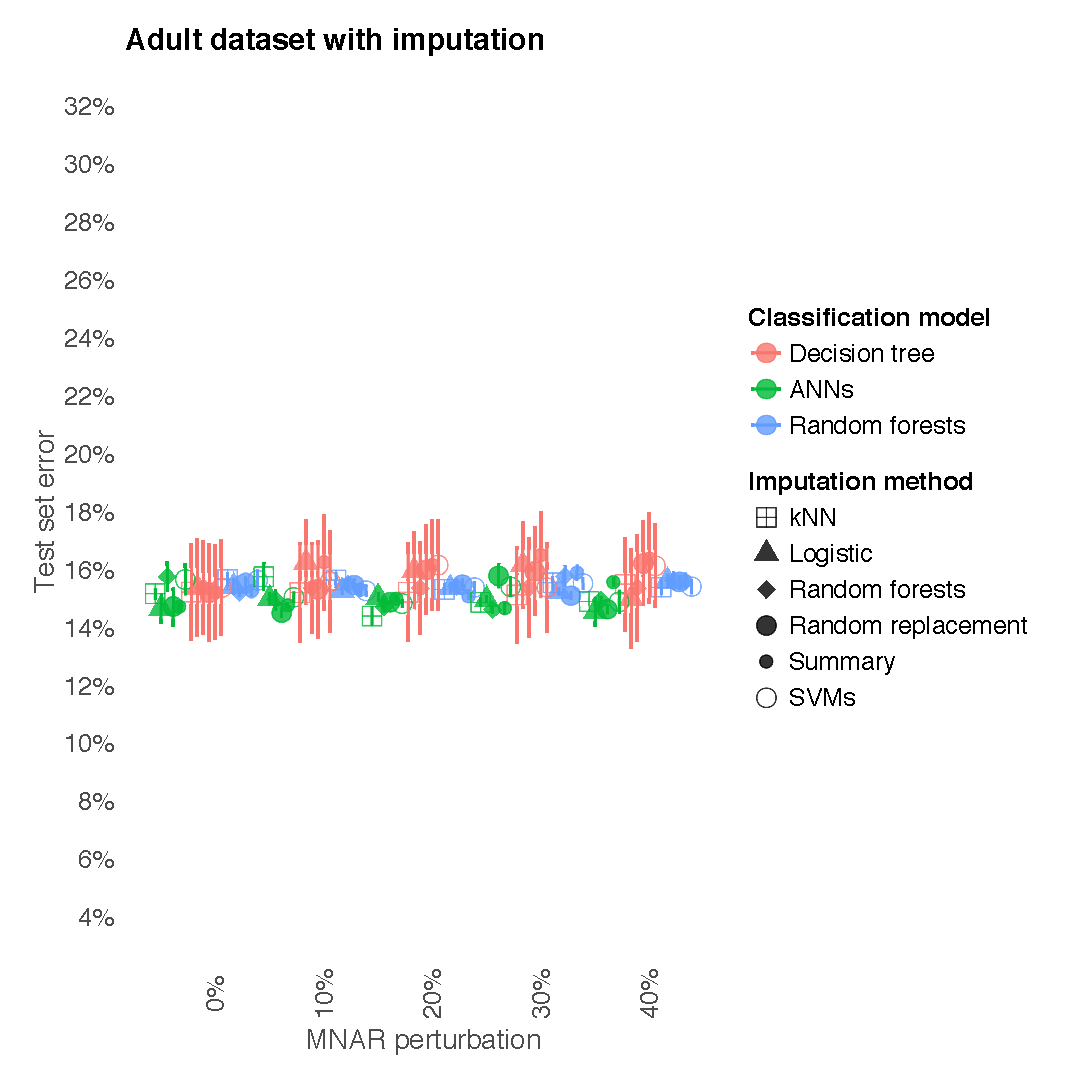
\includegraphics[scale=0.55, center]{figure/test-errors-adult-imp-mnar}\par
   \caption{\footnotesize Error rates on the Adult test set with (bottom) and without (top) missing data imputation, for various levels of MNAR-perturbed categorical training features (x-axis). Error bars represent one standard deviation from the test error prediction.}
   \label{fig:test-error-adult-mnar}
\end{figure}

\begin{figure}[h!]
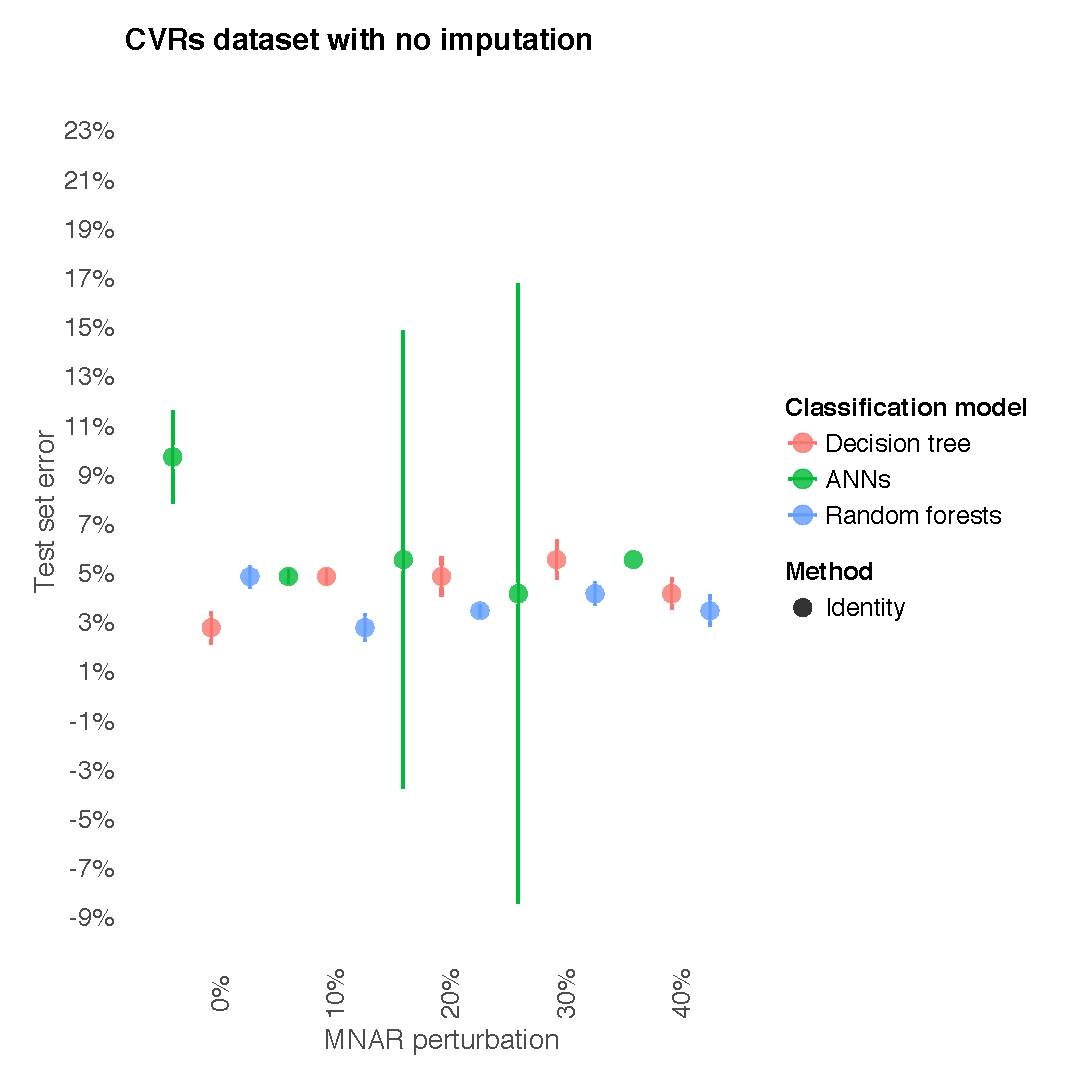
\includegraphics[scale=0.55, center]{figure/test-errors-votes-no-imp-mnar}\par
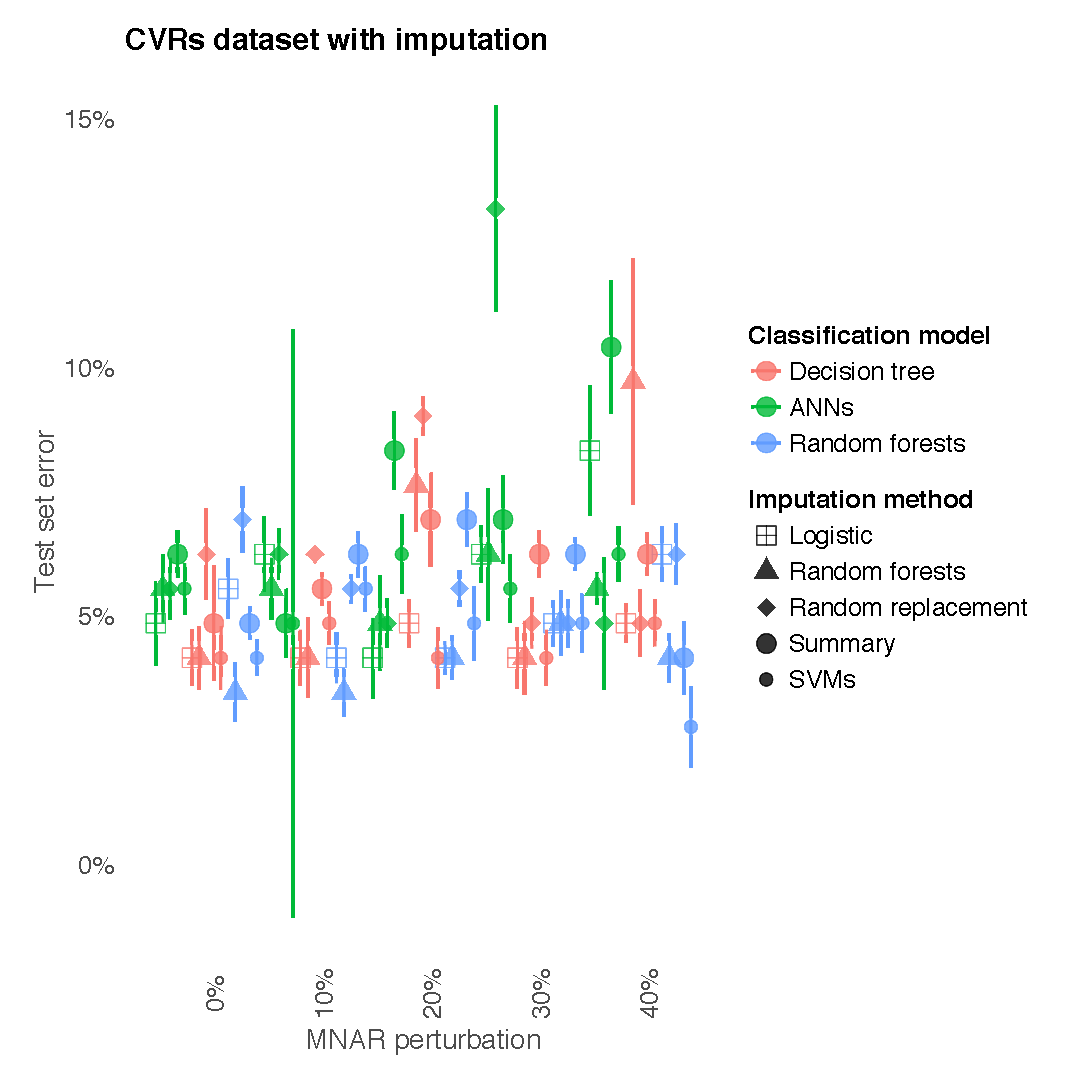
\includegraphics[scale=0.55, center]{figure/test-errors-votes-imp-mnar}\par
   \caption{\footnotesize Error rates on the CVRs test set with (bottom) and without (top) missing data imputation. See footnotes for Figure \ref{fig:test-error-adult-mnar}.}
   \label{fig:test-error-votes-mnar}
\end{figure}

\end{document}
